\begin{figure}[h!]
\centering
\begin{minipage}[b]{0.45\linewidth}
    \centering
    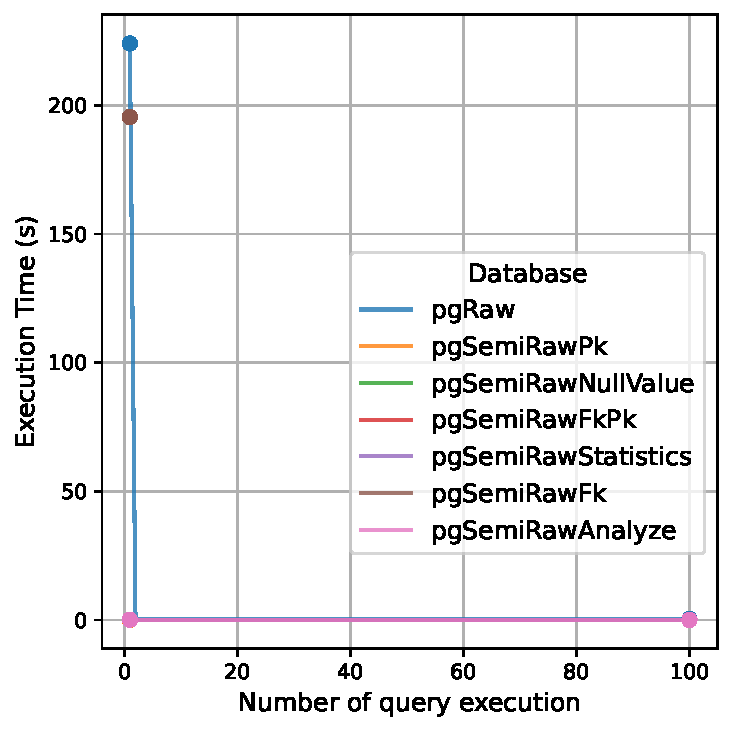
\includegraphics[width=1.0\linewidth]{charts-eval-exp-time/execution_time_db_type_Q5.pdf}
    \caption*{Q5}
\end{minipage}
\hfill
\begin{minipage}[b]{0.45\linewidth}
    \centering
    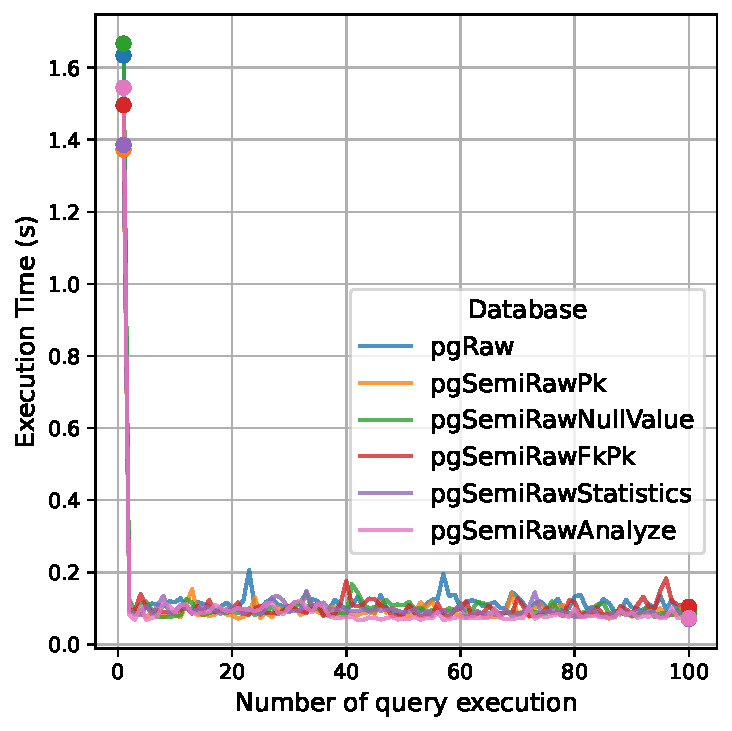
\includegraphics[width=1.0\linewidth]{charts-eval-exp-time/execution_time_db_type_Q6.pdf}
    \caption*{Q6}
\end{minipage}
\vspace{0.5cm}
\begin{minipage}[b]{0.45\linewidth}
    \centering
    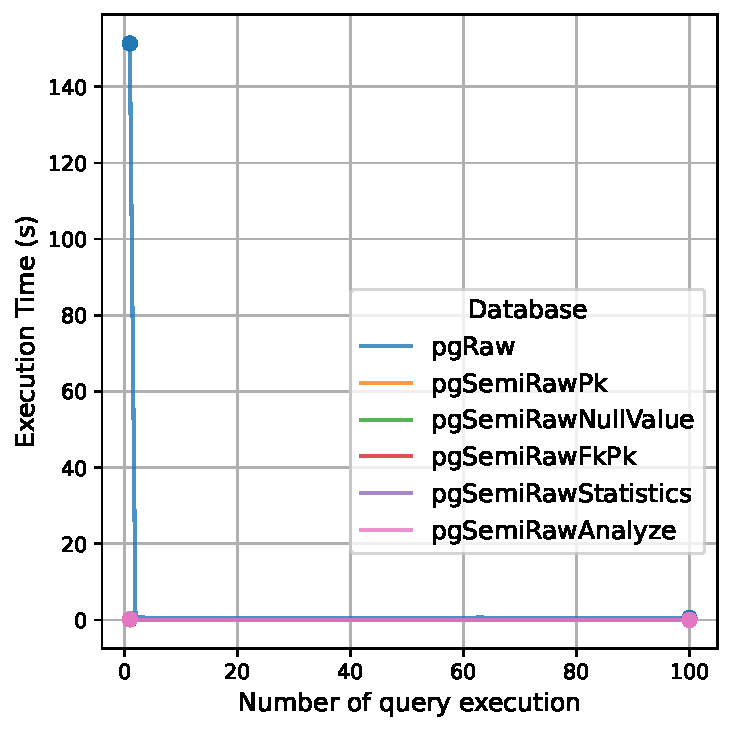
\includegraphics[width=1.0\linewidth]{charts-eval-exp-time/execution_time_db_type_Q7.pdf}
    \caption*{Q7}
\end{minipage}
\hfill
\begin{minipage}[b]{0.45\linewidth}
    \centering
    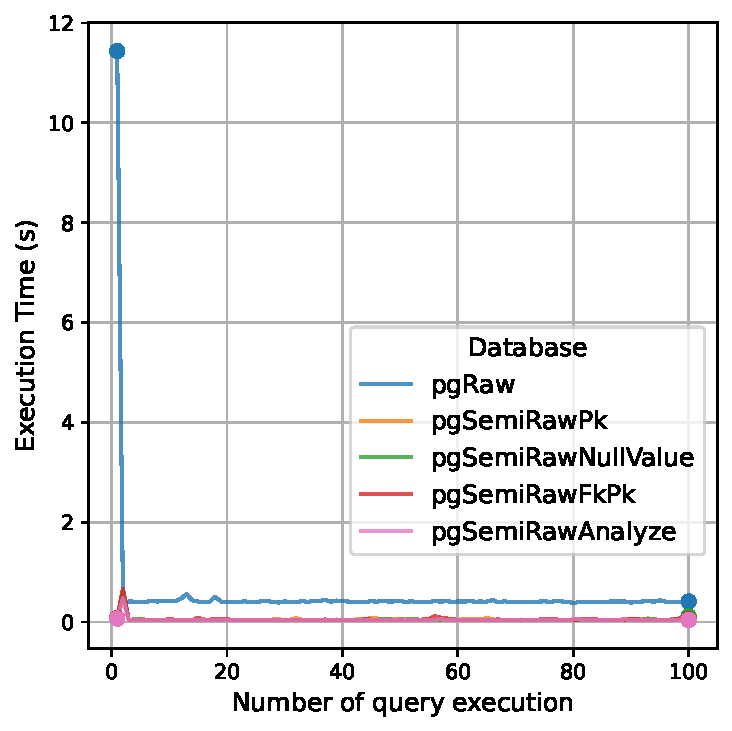
\includegraphics[width=1.0\linewidth]{charts-eval-exp-time/execution_time_db_type_Q9.pdf}
    \caption*{Q9}
\end{minipage}
\caption[The execution times for queries Q5, Q6, Q7, and Q9 over 100 iterations]{The execution times for queries Q5, Q6, Q7, and Q9 over 100 iterations using various types of PostgresSemiRaw and PostgresRaw. These databases include TPC-H data with the \acrshort{sf} 0.1 alongside different levels of metadata.}
\label{fig:execution_time_group2}
\end{figure}
